\documentclass[border=5pt]{standalone}
\usepackage{tikz}
\usepackage{amsmath}
\usetikzlibrary{positioning, arrows.meta, calc, fit, backgrounds, decorations.pathreplacing}

% --- Color Scheme (Blue-Gray) ---
\definecolor{bgPrimary}{HTML}{DAE8FC}
\definecolor{bgSecondary}{HTML}{E8EEF7}
\definecolor{bgAccent}{HTML}{B3CDE3}
\definecolor{bgInput}{HTML}{F0F4F8}
\definecolor{borderPrimary}{HTML}{6C8EBF}
\definecolor{borderAccent}{HTML}{3A6EA5}
\definecolor{arrowColor}{HTML}{4A6A8A}
\definecolor{textMain}{HTML}{2C3E50}
\definecolor{textLight}{HTML}{7F8C8D}
\definecolor{bgHighlight}{HTML}{FFF3CD}

% --- Styles ---
\tikzset{
  module/.style={
    draw=borderPrimary, fill=bgPrimary, rounded corners=4pt,
    minimum width=2.5cm, minimum height=1.0cm,
    font=\sffamily\small, text=textMain, line width=0.6pt, align=center,
  },
  novelmodule/.style={
    draw=borderAccent, fill=bgAccent, rounded corners=4pt,
    minimum width=2.5cm, minimum height=1.0cm,
    font=\sffamily\small\bfseries, text=textMain, line width=1.0pt, align=center,
  },
  iobox/.style={
    draw=borderPrimary, fill=bgInput, rounded corners=3pt,
    minimum width=2cm, minimum height=0.8cm,
    font=\sffamily\small, text=textMain, line width=0.5pt, align=center,
  },
  groupbox/.style={
    draw=borderPrimary, fill=bgSecondary, fill opacity=0.3,
    rounded corners=6pt, inner sep=10pt, line width=0.5pt, dashed,
  },
  stdarrow/.style={
    -{Stealth[length=5pt, width=4pt]}, line width=0.6pt, color=arrowColor,
  },
}

\begin{document}
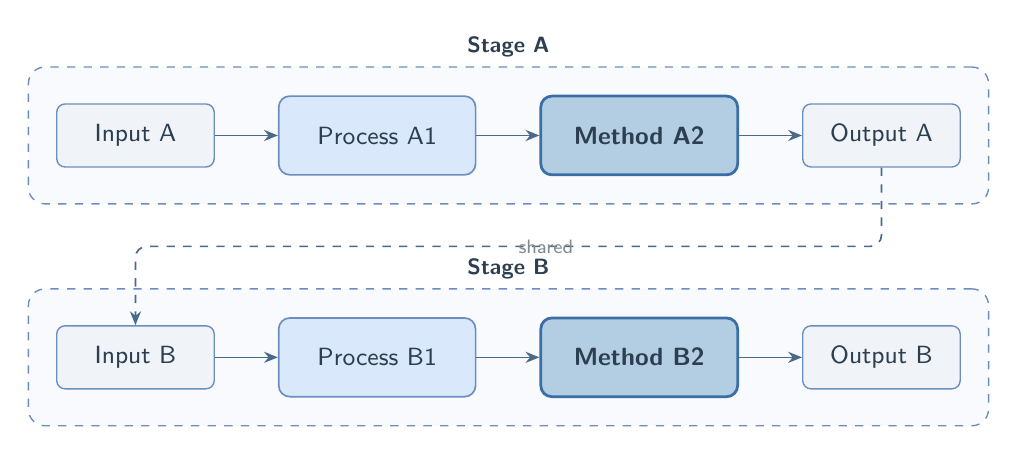
\begin{tikzpicture}

  % === Stage A (top) ===
  \node[iobox]      (inA) {Input A};
  \node[module, right=0.8cm of inA]      (a1) {Process A1};
  \node[novelmodule, right=0.8cm of a1]  (a2) {\textbf{Method A2}};
  \node[iobox, right=0.8cm of a2]        (outA) {Output A};

  \draw[stdarrow] (inA) -- (a1);
  \draw[stdarrow] (a1) -- (a2);
  \draw[stdarrow] (a2) -- (outA);

  % Group box for Stage A
  \begin{scope}[on background layer]
    \node[groupbox, fit=(inA)(a1)(a2)(outA),
      label={[font=\sffamily\footnotesize\bfseries, text=textMain]above:Stage A}] {};
  \end{scope}

  % === Stage B (bottom) ===
  \node[iobox, below=2.0cm of inA]        (inB) {Input B};
  \node[module, right=0.8cm of inB]       (b1) {Process B1};
  \node[novelmodule, right=0.8cm of b1]   (b2) {\textbf{Method B2}};
  \node[iobox, right=0.8cm of b2]         (outB) {Output B};

  \draw[stdarrow] (inB) -- (b1);
  \draw[stdarrow] (b1) -- (b2);
  \draw[stdarrow] (b2) -- (outB);

  % Group box for Stage B
  \begin{scope}[on background layer]
    \node[groupbox, fit=(inB)(b1)(b2)(outB),
      label={[font=\sffamily\footnotesize\bfseries, text=textMain]above:Stage B}] {};
  \end{scope}

  % === Optional connection between stages ===
  \draw[stdarrow, dashed, rounded corners=4pt]
    (outA.south) -- ++(0, -1.0cm)
    -| node[near start, right, font=\sffamily\scriptsize, text=textLight] {shared} (inB.north);

\end{tikzpicture}
\end{document}
